\section*{Описание экспериментальной установки}

\begin{figure}[H]
	\centering
	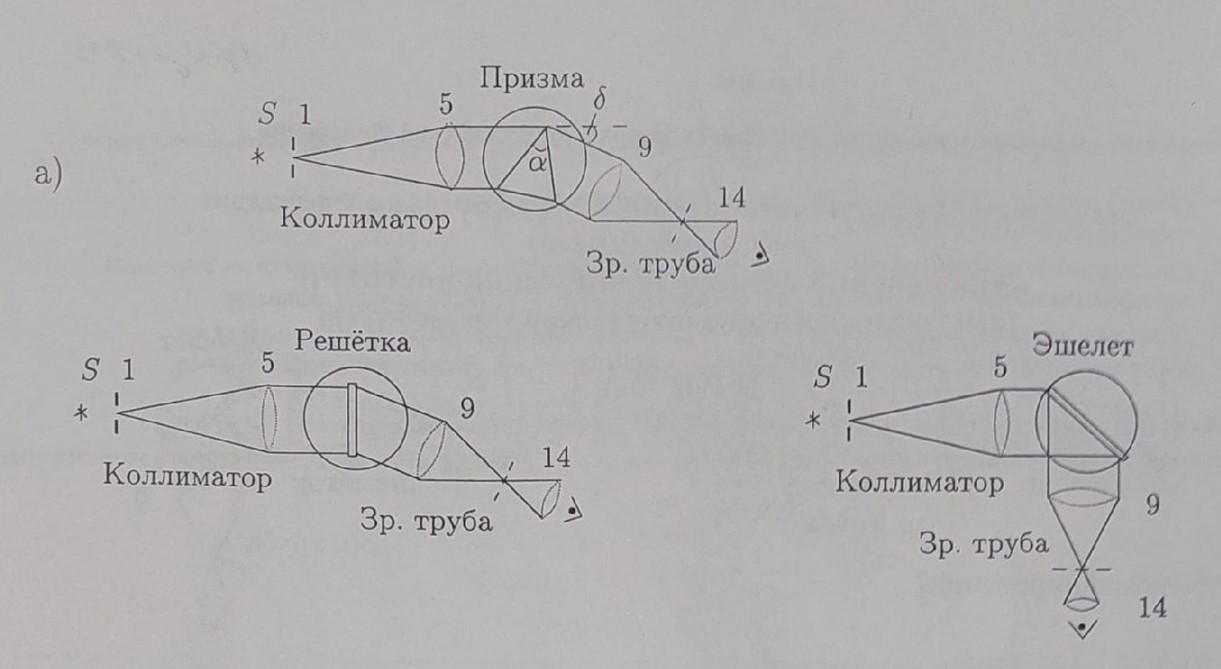
\includegraphics[width=1\textwidth]{../Изображения/Оптические схемы.jpeg}
	\caption{Оптические схемы}
\end{figure}

Внешний вид гониометра представлен на рис. 2б и 2в. Коллиматор 3, столик 7 и алидада 17 со зрительной трубой 12 крепятся на массивном основании 23. На столике 7 размещаются исследуемые объекты. Коллиматор закреплён неподвижно, а столик и алидада с трубой могут вращаться вокруг вертикальной оси.

\begin{figure}[H]
	\centering
	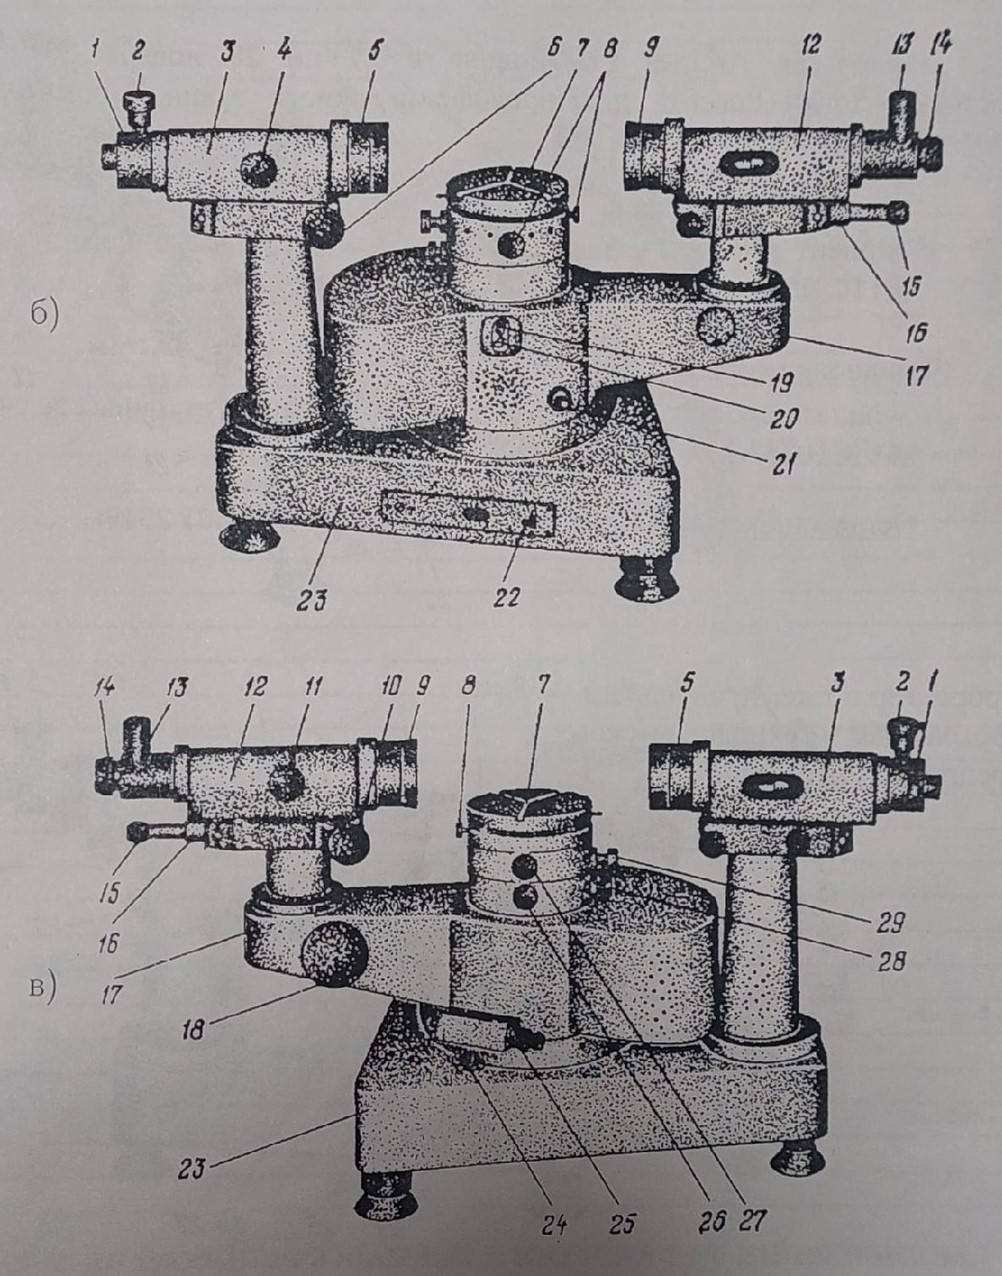
\includegraphics[width=0.8\textwidth]{../Изображения/Внешний вид гониометра.jpeg}
	\caption{Внешний вид гониометра}
\end{figure}

Свет от источника S проходит через коллиматор (щель 1 и объектив 5) и преобразуется призмой в набор параллельных пучков, каждый из которых соответствует определенной длине волны. Параллельные пучки собираются в фокальной плоскости объектива 9 зрительной трубы и рассматриваюстся глазом через окуляр 14.

